% $Id: Z06.tex,v 1.1 2007-02-10 17:22:16 doros Exp $

% This program can be redistributed and/or modified under the terms
% of the Creative Common Licence

\documentclass{beamer}

%\usepackage[headheight=12pt]{beamerthemeboxes}
%\usepackage{beamerthemesplit}
%\usepackage{graphics}

\beamertemplateshadingbackground{red!10}{blue!10}

\usepackage{beamerthemeshadow}

\usepackage[italian]{babel}
%\usepackage{pgf,pgfarrows,pgfnodes,pgfautomata,pgfheaps}
%\usepackage{amsmath,amssymb}
%\usepackage[latin1]{inputenc}
%\usepackage{times}
\usepackage{palatino}

\usepackage{hyperref}

% Use some nice templates

\beamertemplateshadingbackground{red!10}{structure!10}
\beamertemplatetransparentcovereddynamic
\beamertemplateballitem
\beamertemplatenumberedballsectiontoc



\title{Netkit4TIC: il laboratorio virtuale per lo studio di reti}
\author{Sandro Doro}
\institute[ITIS ``C.Zuccante'' - Venezia--Mestre]{
  ITIS ``C.Zuccante'' - Venezia--Mestre\\
  Corso Serale Sirio}
%       Linux registered user n. 5768
%\date{\today}
\date{14 Febbraio 2007}

\AtBeginSection[]{\frame{\frametitle{Programma}\tableofcontents[current]}}



\pgfdeclaremask{tu}{uml-small-mask}
\pgfdeclareimage[mask=tu,width=1cm]{tu-logo}{uml-small}

\logo{\pgfuseimage{tu-logo}}



\begin{document}

%\frame{\maketitle}
\frame{\titlepage
%  \footnotetext{Prodotto con \LaTeX e pdf\LaTeX}
}

\section*{Programma}
\frame{\frametitle{Programma}\tableofcontents[part=1]}



\part{Main part}

%\frame{\partpage}

\section{La virtualizzazione}
\frame{
  \frametitle{La virtualizzazione}
  \begin{block}{Introduzione}

  \begin{itemize}
    \item
  Nel settore dei computer la virtualizzazione \`{e} una tecnica
  per nascondere le caratteristiche fisiche delle risorse
  computazionali.

    \item
  Da alcuni anni si stanno diffondendo progetti il cui scopo \`{e}
  quello di simulare altri sistemi, sia hardware che software.

    \item
  La virtualizzazione di una intera macchina apre nuovi
  scenari nella sperimentazione con il software.
    \item
  Questa idea non \`{e} nuova poich\`{e}
  risale all'epoca d'oro dei mainframe.
  \end{itemize}
  \end{block}

}
\frame{
  \frametitle{Elenco implementazioni}
  \begin{block}{http://en.wikipedia.org/wiki/Virtual\_machine}
  L'elenco \`{e} molto lungo e quindi citeremo solo una parte:
  \begin{itemize}
    \item
    Xen (http://www.cl.cam.ac.uk/Research/SRG/netos/xen/)
    \item
    VMware (http://www.vmware.com/)
    \item
    Virtual Server e Virtual PC (http://www.microsoft.com/whdc/system/platform/virtual/default.mspx)
    \item
    QEMU (http://fabrice.bellard.free.fr/qemu/)
    \item
    Bochs (http://bochs.sourceforge.net)
  \end{itemize}

  \end{block}
}
\frame{
  \frametitle{Supporto Hardware}
  \begin{block}{http://en.wikipedia.org/wiki/Intel\_Virtualization\_Technology}
  
  La Intel e la AMD hanno sviluppato indipendentemente delle
  estensioni alla archittettura x86 per la virtualizzazione:

  \begin{itemize}
    \item
  La tecnologia Intel VT \`{e} disponibile sui processori
  Pentinum 4 6x2, Pentium D 9x0, Xeon 3xxx/5xxx/7xxx, Core Duo
  e Core Duo 2.

    \item
  La tecnologia AMD Virtualization \`{e} disponibile sui processori
  che usano il Socket AM2, Socket S1 e Socket F. \`{E} disponibile
  anche su Athlon 64 e Turion 64.
  \end{itemize}
  \end{block}
}
\subsection{UML}
\frame{
  \frametitle{User Mode Linux}
  \begin{block}{http://www.user-mode-linux.org}
  Il progetto \`{e} ospitato sul sito sourgeforge.net e il suo
  ideatore e autore \`{e} Jeff Dike. Si \`{e} laureato al MIT
  e in seguito ha lavorato presso la Digital fino al 1993.
  Nel decennio successivo ha lavorato come
  indipendente ed  \`{e} diventato un Linux kernel developer
  nel 1999. Dal 2004 lavora presso la Intel.
  Contribuisce al progetto
  anche un giovane italiano: Paolo Giarrusso.\\

  A partire dalla versione 2.6.0 \`{e} parte integrante del
  kernel di Linux.\\

  \end{block}
}
\frame{
  \frametitle{User Mode Linux - caratteristiche}
  \begin{itemize}
    \item Permette di eseguire multipli sistemi Linux (indicati
          come "guest") in un normale sistema Linux (indicato come
          "host") ossia
          da un pc con installato GNU/Linux posso ``creare'' un altro
          sistema GNU/Linux anche di una diversa distribuzione.\\
    \item \`{E} un sistema di virtualizzazione di tipo emulativo
          ossia ha lo scopo di riprodurre accuratamente le
          \textbf{funzionalit\`{a}} di un sistema reale ma con
          una limitata velocit\`{a}.
  \end{itemize}
}
\frame{
  \frametitle{User Mode Linux - come lavora}
          Un programma che necessita dell'uso dell'hardware
          (scheda video, tastiera, ecc) richiede il servizio
          al kernel. Nel caso di utilizzo di UML la richiesta viene
          fatta al kernel User Mode Linux:
  \begin{center}
  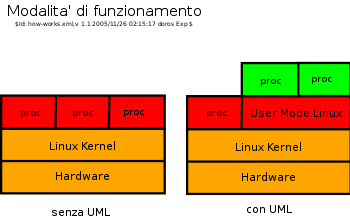
\includegraphics[width=7cm]{how-works.png}
  \end{center}
}
\subsection{QEMU}
\frame{
  \frametitle{QEMU processor emulator}
  \begin{block}{http://fabrice.bellard.free.fr/qemu/}
  Il progetto \`{e} ideato e coordinato dal francese
  Fabrice Bellard. \`{E} un emulatore multipiattaforma che
  permette di eseguire del codice Linux compilato per una
  particolare CPU su di un processore x86: per esempio
  codice SPARC o ARM.\\
  Per avere una maggire velocit\`{a} deve essere compilato
  anche il modulo acceleratore kqemu.
  \end{block}
}
\subsection{Applicazioni}
\frame{
  \frametitle{Applicazioni}
  I contesti in cui si utilizza la virtualizzazione di un intero sistema
  operativo sono ad esempio:

  \begin{itemize}
    \item Ambiente di testing di nuovo software
    \item Ambiente di simulazione di protocolli di rete
    \item Costruzione di Honeynet virtuali
    \item Costruzione di Virtual Host per Hosting Service
    \item Costruzione di Virtual Cluster con OpenMosix
  \end{itemize}
}
\frame{
  \label{test (1)}
  \frametitle{UML - Ambiente di testing di nuovo software (1)}
  Il progetto OpenSWAN (IPsec per Linux):
  \begin{itemize}
    \item si basa su righe di codice
  estremamente complicate per la comunicazione in rete
    \item cifra tutto il traffico di rete
    \item Utilizza un sistema
  di chiavi dinamico che rende praticamente impossibile ad un osservatore
  di capire cosa viene trasmesso
    \item occorrono circa 6
  sistemi per testare completamente il codice prodotto e quindi \`{e}
  impossibile o troppo costoso tenere un tale sistema dispobile
  solo per questo scopo
  \end{itemize}
}
\frame{
  \label{test (2)}
  \frametitle{UML - Ambiente per testing di nuovo software (2)}
  Il progetto BorpLAN:
  \begin{itemize}
    \item si tratta di una applicazione ``web based'' realizzata
  come stage estivo A.S. 2005
  da Simone Veronese ex studente dell'ITIS ``C.Zuccante'' di Mestre (VE) e
  finanziata dalla Cassa di Risparmio di Venezia. Lo scopo
  della applicazione \`{e} costruire un sistema capillare
  di controllo degli accessi alla rete tramite l'uso di un browser e
  di packet filter.
    \item 
  per testare completamente il codice prodotto 
  occorrono almeno 2 router, 2 pc client e un web server
  e quindi \`{e}
  difficile e costoso mettere a disposizione una tale struttura. Inoltre
  nel caso di bugs il sistema deve risultare pronto per l'accettazione
  e la verifica del bug stesso e per la successiva risoluzione.
  \end{itemize}
}
\frame{
  \label{simu}
  \frametitle{Ambiente di sperimentazione di protocolli di rete}
  Il progetto UMTS/TIC corsi C1 e C2 \`{e} un progetto del MIUR
  per la formazione del personale interno (ATA e docenti) sulla
  infrastruttura tecnologica.\\
  Si sono verificati alcuni problemi:
  \begin{itemize}
    \item mancanza di un laboratorio creato appositamente e sempre accessibile
    ai corsisti per effettuare le loro prove
    \item mancanza di un sufficiente numero di computer
    \item impossibilit\`{a} di effettuare le esercitazioni a casa
  \end{itemize}
}
\frame{
  \frametitle{Laboratorio di sistemi/informatica}
  Negli istituti tecnici a indirizzo informatica (ABACUS/Sirio)
  nell'ultimo anno di corso, a volte anche prima, si studiano
  le reti e le applicazioni web. Per l'assimilizione effettiva
  da parte degli studenti sarebbe opportuno:
  \begin{itemize}
    \item mettere a disposizione \textbf{per ogni studente} un gruppo di sistemi
          da configurare e amministrare
    \item avere lo stesso sistema \textbf{a casa}
  \end{itemize}
}
\frame{
  \frametitle{Costruzione di Honeynet (vasi di miele)}
  Gli Honeynet sono dei sistemi installati sulle reti e servono per attirare
  eventuali intrusi e per studiare le loro mosse.
  Queste reti
  di sistemi sono altamente controllate e quando uno dei sistemi
  \`{e} attaccato esso cattura tutta l'attivit\`{a} dell'intruso.
  Un articolo che spiega come costruirli \`{e}:
  \href{http://www.honeynet.org/papers/virtual/}{``Know Your Enemy: Defining Virtual Honeynets''}
  tradotti in italiano in una serie di tre articoli(
  \href{http://www.honeynet.org/papers/trans/nemico.html}{1},
  \href{http://www.honeynet.org/papers/trans/nemico2.html}{2},
  \href{http://www.honeynet.org/papers/trans/nemico3.html}{3})
}
\frame{
  \frametitle{Costruzione di Virtual Host per Hosting Service}
  La vendita di servizi di hosting \`{e} un mercato in forte crescita
  e spesso chi li utilizza desidera passare dalla soluzione
  di delega della gestione dei propri servizi al pieno possesso
  degli stessi per ottenere pi\`{u} flessibilit\`{a}.
  La soluzione pi\`{u} vantaggiosa \`{e} sicuramente l'acquisto
  di un sistema virtuale.
  Un articolo che racconta la nascita di un provider di questo tipo \`{e}:
  \href{http://uml.openconsultancy.com/}{``UML-based pseudo-dedicated hosting service''}
}
\frame{
  \begin{center}
  
\includegraphics[width=3cm]{OpenMosix.jpg}
  \end{center}
  \frametitle{Costruzione di Cluster con OpenMosix}
  OpenMosix \`{e} un progetto Open Source che estende il
  kernel di Linux per costruire cluster basati su una
  singola immagine. Una fotografia di un cluser \`{e} visibile sullo
  \href{http://www.mosixview.com/umopenmosix/umopenmosix.jpg}{screenshot}.
  Un articolo che descrive come costruire un cluster UML OpenMosix \`{e}:
  \href{http://www.mosixview.com/umopenmosix/umopenmosix.html}{``User Mode openMosix: a virtual openMosix cluster running in User-mode''}
}





\section{Netkit}
\frame{
  \frametitle{Cos'\`{e} Netkit - http://www.netkit.org}
    Netkit \`{e} il risultato del lavoro di alcune persone del
    Networks Research Group dell'Universit\`{a} di Roma 3 e
    del Linux User Group LUG Roma 3. Il software \`{e} composto da:
  \begin{itemize}
    \item Un insieme predefinito di comandi per il setup di
          macchine virtuali
    \item Un filesystem con preinstallato il software
          necessario per le sperimentazioni
  \end{itemize}
}
\subsection{Linee guida}
\frame{
  \frametitle{Linee guida}
  Netkit \`{e} stato concepito come un ambiente a basso costo per
  esperimenti di rete. All'interno del suo ambiente possono essere
  ``creati'' e interconessi dei completi router, switch e host. Tali
  apparati sono virtuali ma possono operare con molte delle
  caratteristiche possedute da quelli reali.
}
\frame{
  \frametitle{Considerazioni generali}
  \begin{itemize}
    \item Basato su User Mode Linux
    \item Ogni apparato di rete \`{e} una linux box
    \item Linux supporta quasi tutti i protocolli di rete
          e pu\`{o} essere configurato come bridge/switch o
          come router
  \end{itemize}
}
\frame{
  \frametitle{Struttura}
  \begin{itemize}
    \item Le varie istanze che simulano gli apparati di rete
          sono create all'interno dello stesso host
    \item Le varie istanze sono interconnesse in domini di
          collisione (hub/switch)
    \item Il ruoli dei nodi sono configurabili
  \end{itemize}
}
\subsection{Esperienze riproducibili}
\frame{
  \frametitle{Esperienze riproducibili}
  \begin{itemize}
    \item Esperienze base: rete minimale con due host, tabelle di routing,
          protocollo ARP, protocollo RIP.
    \item Esperienze applicative: configurazione di DNS e Mail server.
    \item Esperienze avanzate: esperienze su switch e STP.
    \item Esperienze su routing interdomio (bgp): routing tra Autonomous
          System.
  \end{itemize}
}
\subsection{NetML: Network Markup Language}
\frame{
  \frametitle{http://www.dia.uniroma3.it/\~\space compunet/netml}
  \begin{itemize}
    \item \`{E} un linguaggio di marcatori per la descrizione
          e la configurazione di reti. \`{E} basato su XML.
          Principalmente pensato per descrivere reti di
          Autonomous System o per la descrizione delle reti
          a livello 2 ISO/OSI.
    \item Attraverso XSLT \`{e} possibile produrre i file di
          configurazione per alcuni tipi di router e recentemente
          \`{e} stata aggiunta la possibilit\`{a} di esprimere
          regole di firewall.
  \end{itemize}
}




\section{Netkit4TIC}
\frame{
  \frametitle{Netkit4TIC - http://www.tic.fdns.net/tic/html/lab.html}
  Questo progetto \`{e} nato nel 2003 dalla necessit\`{a} nei
  corsi UMTS/TIC C2 di un laboratorio
  di sperimentazione ``permanente''.\\
  Le aree di interesse, intersecate tra loro, si possono
  dividere in:
  \begin{itemize}
    \item problematiche di rete: lo stack TCP/IP e la
          progettazione in generale di reti
    \item configurazione servizi: Web, DNS, 
          directory services, file share, Kerberos, Terminal Server
    \item problematiche sulla sicurezza: cifratura,
          certificati elettronici, VPN
  \end{itemize}
}
\subsection{Struttura}
\frame{
  \frametitle{Struttura}
  \`{E} composto da due parti:
  \begin{enumerate}
    \item Live-\{CD,USB\}: \`{e} una distribuzione GNU/Linux in grado di
          ``eseguire'' le esperienze senza bisogno di installazione. Contiene:
    \begin{itemize}
      \item una versione di Knoppix elaborata per ottenere migliori
            prestazioni con UML.
      \item un kernel UML e un filesystem con preinstallato una parte
            della distribuzione GNU/Linux Debian sarge
      \item un kernel UML e un filesystem con la distribuzione LEAF/Bering con
            librerie uClibc per sistemi embedded.
      \item una versione leggermente personalizzata di Netkit
    \end{itemize}
    \item Internet: dal sito
          \href{http://www.tic.fdns.net/tic/html/lab.html}{http://www.tic.fdns.net/tic/html/lab.html}
          sono scaricabili le esperienze virtuali (qualche Kbyte) in formato archivio compresso (tgz).
  \end{enumerate}
}
\subsection{Esperienze riproducibili}
\frame{
  \frametitle{lo stack TCP/IP e la progettazione di reti}
  \begin{block}{Esperienze riproducibili}
  \begin{itemize}
    \item bridge, Bridge+STP, VLAN, proxyARP
    \item tabella di routing (statica), protocollo OSPF, Controllo LAB
    \item Qualit\`{a} del Servizio (QoS)
    \item Esercizi: NetPractice
  \end{itemize}
  \end{block}
}
\frame{
  \frametitle{Web, DNS, directory services, Kerberos, cluster HA, file share, LTSP}
  \begin{block}{Esperienze riproducibili}
  \begin{itemize}
    \item file sharing: Samba, Samba Enterprise e Dual Samba
    \item directory service: OpenLDAP
    \item Kerberos V e Single Sign On
    \item HA-Cluster, AFS, XFS
    \item Terminal Server
    \item Manutenzione reti via SNMP
  \end{itemize}
  \end{block}
}
\frame{
  \frametitle{Sicurezza}
  \begin{block}{Esperienze riproducibili}
  \begin{itemize}
    \item Firewall
    \begin{itemize}
       \item a singola area interna
       \item con area interna e area smilitarizzata (DMZ)
       \item con due are perimetrali e backbone interno
    \end{itemize}
    \item PKI: OpenCA una infrastruttura Open Source 
    \item Protocolli SSH e SSL
    \item VPN
    \item Sistemi di rilevazione intrusioni
  \end{itemize}
  \end{block}
}
\subsection{La nuova release v2.3}
\frame{
  \frametitle{Novit\`{a} della versione 2.3}
  \begin{block}{Kernels UML}
  \begin{itemize}
    \item ver 2.4.27 per la simulazione del nodo Debian Sarge
    \item ver 2.4.33 per la simulazione del nodo Bering uClibc
    \item ver 2.6.11 default netkit (quando non specificato)
  \end{itemize}
  \end{block}
}
\frame{
  \frametitle{selezione nodo Sarge}
  \begin{block}{Variabili d'ambiente}
  \begin{itemize}
    \item selezione del kernel:\\
          NETKIT\_VM\_TYPE=sarge     
  \end{itemize}
  \end{block}
}
\frame{
  \frametitle{selezione nodo Bering}
  \begin{block}{script lab.conf}
  \begin{itemize}
    \item selezione del kernel:\\
          nodo[k]="/usr/local/netkit/kernel/ub.krnl"
    \item selezione del software da installare sul Bering:\\
          nodo[append]=LRP=root,config,etc, ... ,customvm
  \end{itemize}
  \end{block}
}
\frame{
  \frametitle{aggiunta connessione di rete "reale"}
  \begin{block}{parametri}
  \begin{itemize}
    \item default netkit
    \item --append=``ethX=tuntap,tap0''
  \end{itemize}
  \end{block}
}
\subsection{Demo}
\frame{
  \frametitle{Dual Samba: due istanze nello stesso nodo}
  \begin{block}{Fattori caratterizzanti}
  \begin{center}
  \begin{itemize}
    \item Uso contemporaneo di due sistemi di
          virtualizzazione: UML e QEMU
    \item Uso di nodi Linux e nodi Windows
    \item Utilizzo di una doppia istanza di Samba
          (in simulazione di un guasto su un HA-cluster
           di tipo active-active)
  \end{itemize}
  
  \end{center}
  \end{block}
}
\frame[containsverbatim]{
  \frametitle{dual Samba}
  \begin{block}{script esperienza Netkit4TIC}
  \footnotesize
  \begin{verbatim}
$ wget http://www.tic.fdns.net/tic/html/dualSamba.tgz
$ tar zxf dualSamba.tgz
$ cd dualSamba
$ ifname=`sudo tunctl -b -u knoppix`

$ sudo ifconfig $ifname 192.168.77.2
# echo "1" > /proc/sys/net/ipv4/ip_forward
# route add -net 192.168.50.0/24 gw 192.168.77.2

$ ./lab start                        # UML side

$ qemu -m 120 -hda XPPSP2.img        # QEMU side
  \end{verbatim}
  \end{block}
}
\frame{
  \frametitle{screenshot}
  \begin{center}
  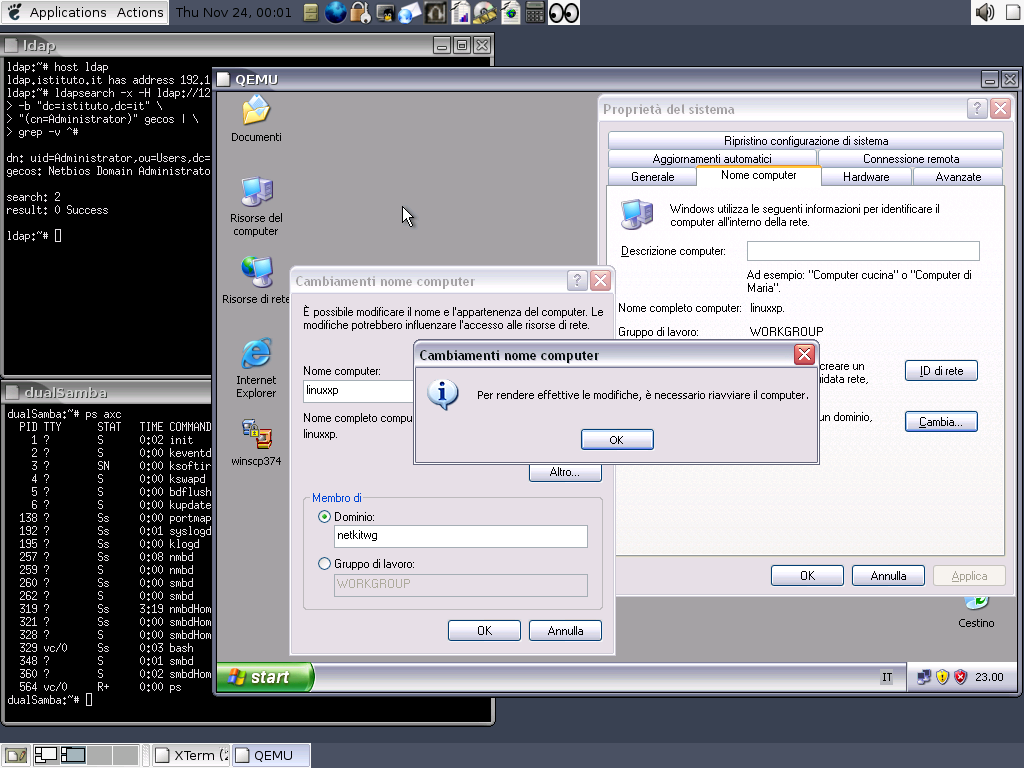
\includegraphics[width=9cm]{XP-dualSamba-09.png}
  \end{center}
}


\section*{Sommario}

\frame{
  \frametitle{Sommario}

  \begin{block}{Riassunto}
  \begin{itemize}
  \item
    Lo studio e la progettazione di reti e di servizi di rete \`{e} un
    elemento essenziale del nostro futuro.
  \item
    La modalit\`{a} dell'apprendimento virtuale \`{e} in grande
    espansione.
  \item
    Esiste una via economica e valida: Netkit4TIC
  \end{itemize}
  \end{block}{}

  \begin{block}{Problemi Aperti}
    \begin{itemize}
    \item
      Adozione
    \item
      Documentazione in lingua inglese.
    \end{itemize}
  \end{block}


}

%\frame{}   % to enforce entries in the table of contents

\end{document}
